\begin{figure*}[t]
    \centering
    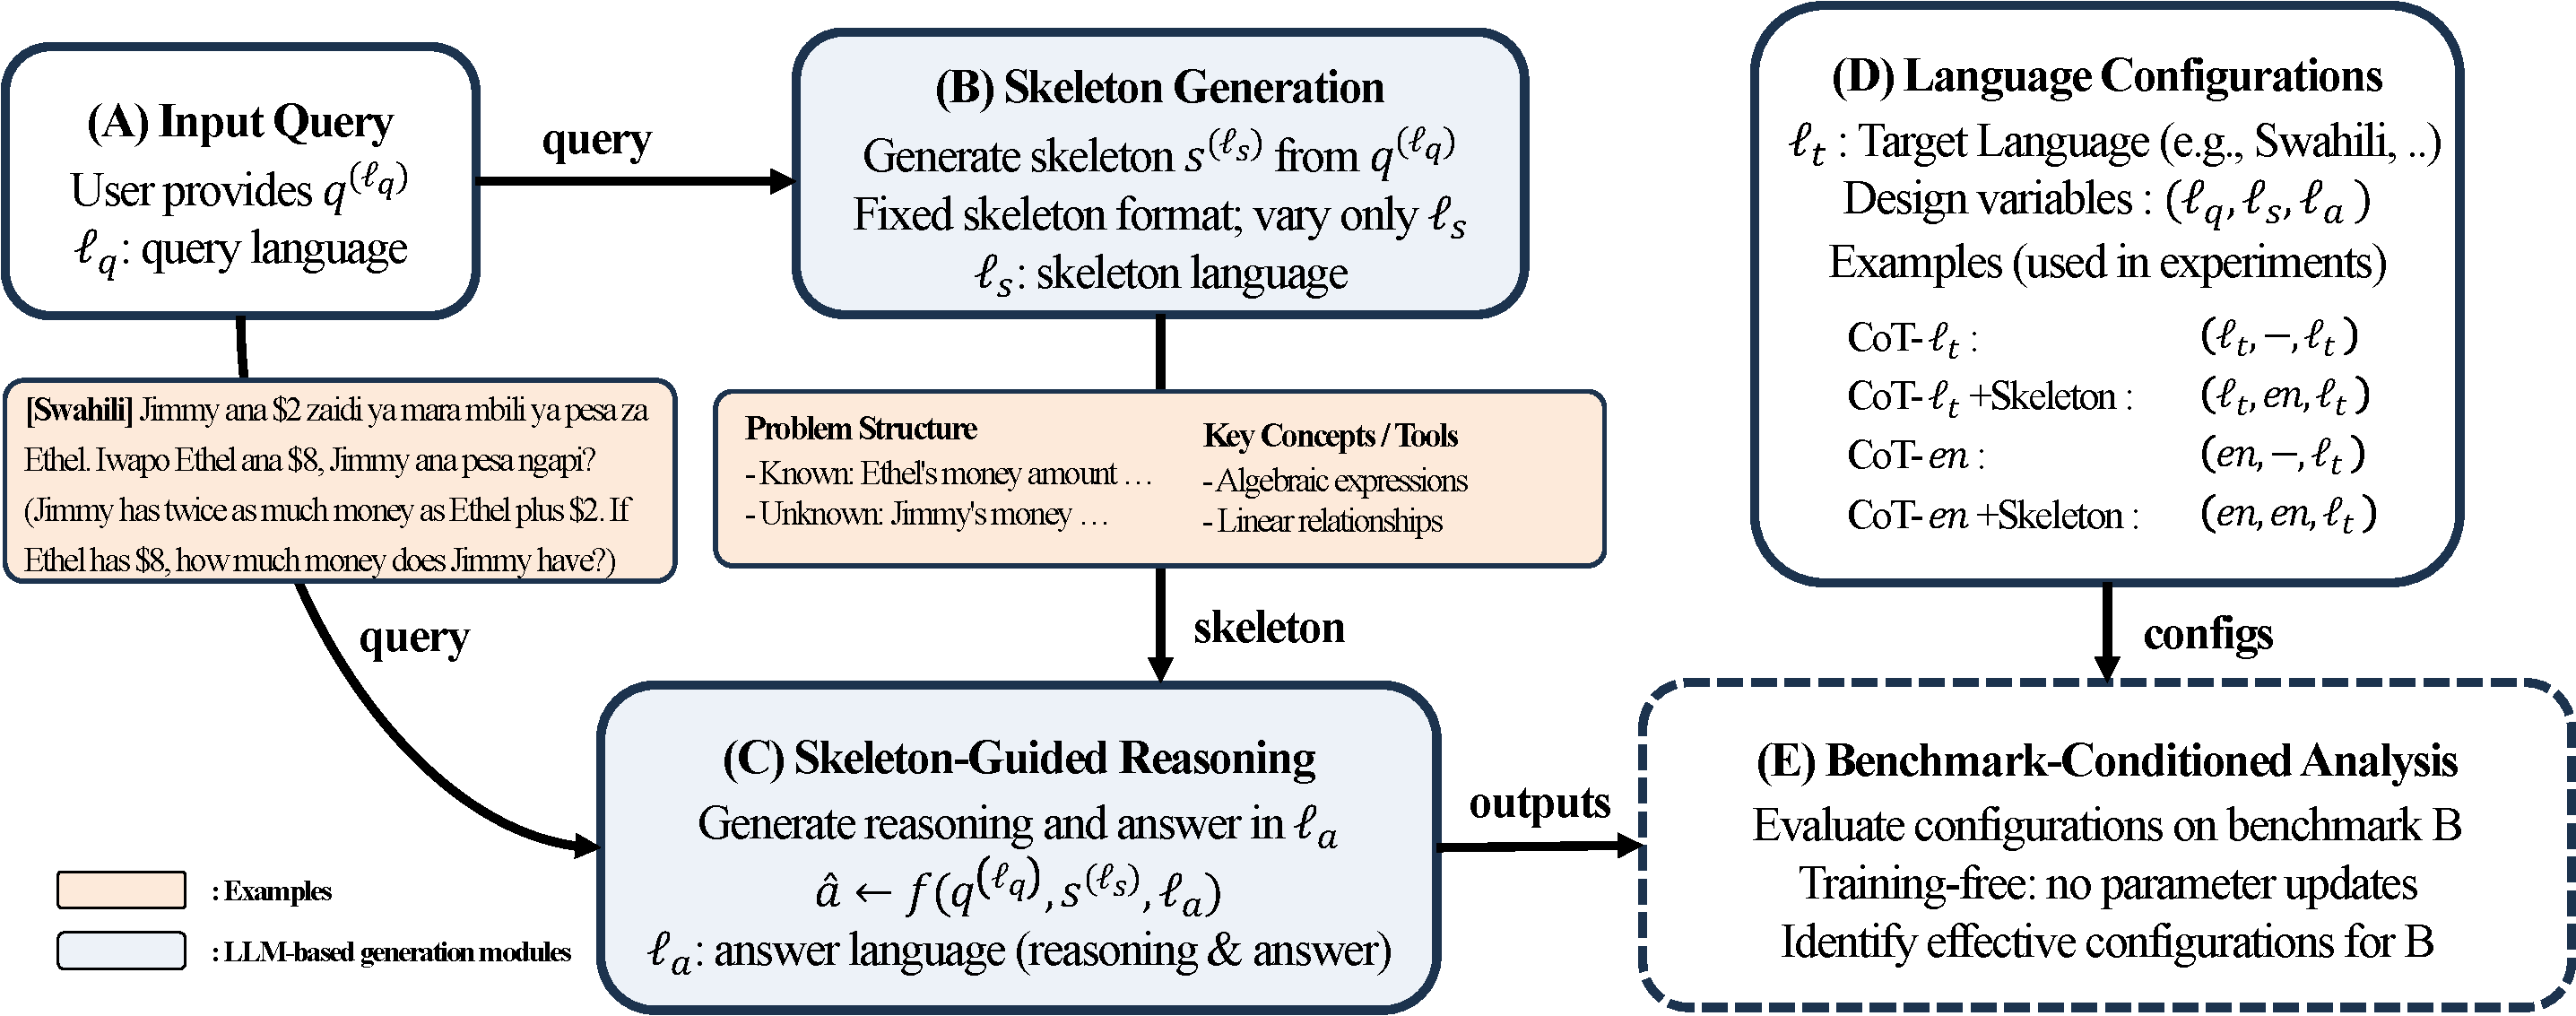
\includegraphics[width=\textwidth]{Figures/Images/LASOF3.pdf}
    \caption{\small Overview of the Skeleton-Guided Reasoning Framework. (A) The process begins with an input query $q^{(\ell_q)}$. (B) A structured skeleton $s^{(\ell_s)}$ is generated to abstract the problem logic. (C) The final reasoning and answer $\hat{a}$ are produced in the answer language $\ell_a$, conditioned on the query and skeleton. (D) We define the language configuration space as $(\ell_q, \ell_s, \ell_a)$ and compare four primary strategies: standard CoT and skeleton-guided approaches, applied in both the target language ($\ell_t$) and English ($en$). (E) Effective configurations are identified through training-free benchmark analysis.
}
\label{fig:figure1}
    \vspace{-0.15in}
\end{figure*}
